%  !TeX  root  =  user_guide.tex

\section{Модуль привязки растров}

% when the revision of a section has been finalized,
% comment out the following line:
%\updatedisclaimer

Модуль привязки растров является инструментом создания файлов привязки
для растровых изображений. Он позволяет ссылаться на географическую или
спроектированную систему координат путем создания нового файла формата
GeoTiff или же объединения файла привязки с существующим изображением.
Основной подход в процессе привязки растров "--- это расположить точки на
изображении, на котором вы можете точно определить их координаты.

\minisec{Кнопки панели инструментов модуля}

\begin{table}[h]\index{Georeferencer!tools}
\begin{tabular}{|m{1cm}|m{6cm}|m{1cm}|m{6cm}|}
 \hline \textbf{Иконка} & \textbf{Назначение} & \textbf{Иконка} &
 \textbf{Назначение} \\
 \hline 
\includegraphics[width=0.7cm]{mActionAddRasterLayer} & Открыть растр &
 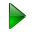
\includegraphics[width=0.7cm]{mActionStartGeoref} & Начать привязку \\
 \hline 
\includegraphics[width=0.7cm]{mActionGDALScript} & Создать сценарий GDAL &
 
\includegraphics[width=0.7cm]{mActionFileOpen} & Загрузить контрольные точки \\
 \hline 
\includegraphics[width=0.7cm]{mActionFileSave} & Сохранить контрольные точки как &
 
\includegraphics[width=0.7cm]{mActionOptions} & Параметры трансформации \\
 \hline 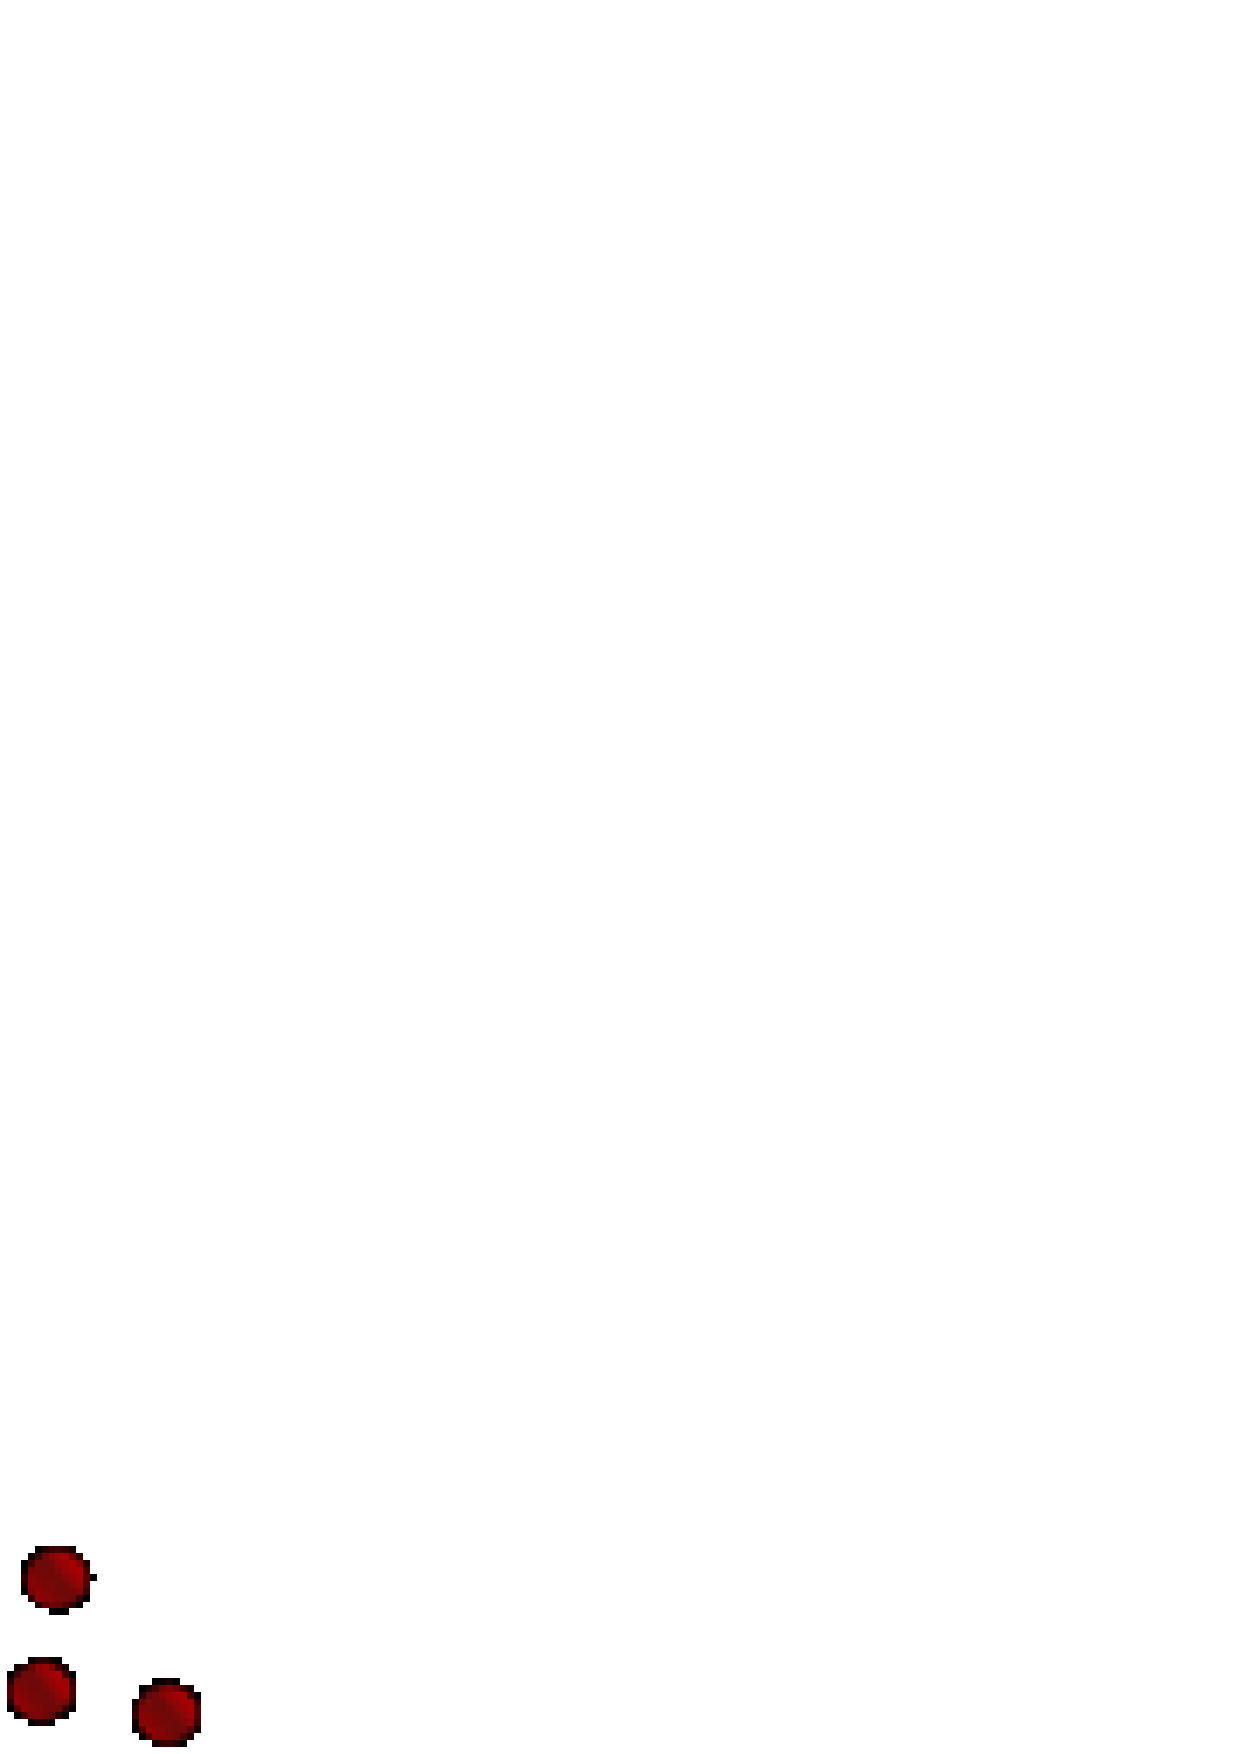
\includegraphics[width=0.7cm]{mActionCapturePoint} & Добавить точку &
 
\includegraphics[width=0.7cm]{mActionDeleteSelected} & Удалить точку \\
 \hline 
\includegraphics[width=0.7cm]{mActionEditPaste} & Переместить точку &
 
\includegraphics[width=0.7cm]{mActionPan} & Прокрутка \\
 \hline 
\includegraphics[width=0.7cm]{mActionZoomIn} & Увеличить &
 
\includegraphics[width=0.7cm]{mActionZoomOut} & Уменьшить \\
 \hline 
\includegraphics[width=0.7cm]{mActionZoomToLayer} & Увеличить до слоя &
 
\includegraphics[width=0.7cm]{mActionZoomLast} & Предыдущий охват \\
 \hline 
\includegraphics[width=0.7cm]{mActionZoomNext} & Следующий охват &
 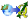
\includegraphics[width=0.7cm]{mActionLinkGeorefToQGis} & Связать модуль привязки растров с QGIS \\
 \hline 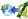
\includegraphics[width=0.7cm]{mActionLinkQGisToGeoref} & Связать QGIS с модулем привязки растров &
 &  \\
\hline
\end{tabular}
\caption{Инструменты привязки растров}\label{tab:georeferencer_tools}
\end{table}

\minisec{Стандартная процедура}

Если имеются координаты X и Y (или же в формате DMS (градусы, минуты,
секунды), DD (десятичная запись), или спроектированные координаты
(mmmm.mm)), соответствующие выбранной точке на изображении, возможно
применение двух альтернативных процедур:

\begin{enumerate}
\item Иногда на самом растровом изображении координаты надписаны.
В таком случае их можно ввести вручную.
\item Использование уже привязанных слоев, векторых или растровых,
содержащих те же самые объекты, которые есть на привязываемом
изображении, а также проекции, подходящей для вашего изображения.
В таком случае, можно ввести координаты в набор опорных данных,
загруженных в QGIS.
\end{enumerate}

Стандартная процедура привязки растровых изображений подразумевает выбор
множественных точек на растре, обозначение их координат или выбор
соответствующего типа преобразования. Исходя из введенных параметров и
данных, модуль вычислит параметры файла привязки. Чем больше координат
будет введено, тем точнее будет результат.

Для начала нужно запустить QGIS, загрузить модуль привязки растров
(см. Раздел~\ref{sec:load_core_plugin}) и нажать на иконку
\toolbtntwo{georeferencer}{Привязка растров}, которая находится на
панели инструментов QGIS. После этого появится диалоговое окно модуля
привязки растров, как показано на рисунке~\ref{fig:georefplugin}.

Для этого примера решено использовать топографическую карту Южной
Дакоты, взятую с сайта Геологического Комитета Южной Дакоты. Позже она
может быть показана вместе с данными выборки GRASS spearfish60. Карту
можно загрузить отсюда:
\url{http://grass.osgeo.org/sampledata/spearfish_toposheet.tar.gz}

\begin{figure}[ht]
\centering
  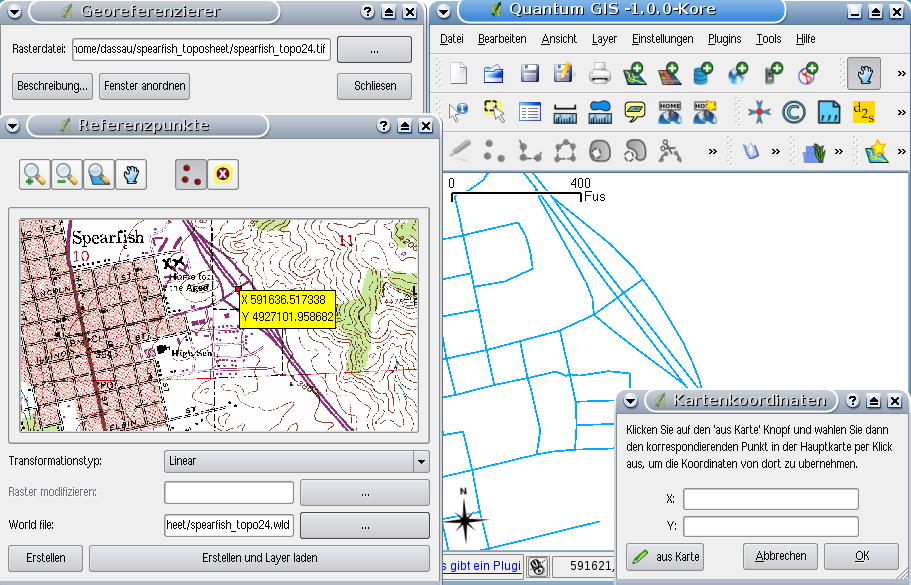
\includegraphics[clip=true, width=12cm]{georefplugin}
  \caption{Диалоговое окно модуля привязки растров \nixcaption}\label{fig:georefplugin}
\end{figure}

\minisec{Ввод контрольных точек}\label{georeferencer_entering}

\begin{enumerate}
\item Для того, чтобы начать привязку непривязанного растрового
изображения, сначала нужно загрузить его, используя кнопку

\includegraphics[width=0.7cm]{mActionAddRasterLayer}. Само растровое
изображение появится в основном рабочем окне диалогового окна модуля.
Как только растр загрузится, можно начинать ввод точек привязки.
\item Используя кнопку \toolbtntwo{mActionCapturePoint}{Добавить точку},
следует добавить точки в основном рабочем окне и ввести их координаты
(см. Рисунок~\ref{fig:choose_points}). Данную операцию можно проделать
двумя путями:

\begin{enumerate}
\item Щелкнуть мышью по точке на растровом изображении и ввести
координаты X и Y вручную
\item Щелкнуть мышью по точке на растровом изображении и нажать кнопку
\toolbtntwo{pencil}{с карты} для того, чтобы добавить координаты X и Y
с помощью привязанной карты, уже загруженной в QGIS.
\end{enumerate}
\item Продолжить ввод точек. Необходимо как минимум 4 точки, и чем
больше координат можно ввести, тем точнее будет результат. В диалоговом
окне модуля есть дополнительные инструменты для увеличения/уменьшения
или прокрутки рабочего окна для того, чтобы определить соответствующий
набор контрольных точек.
\end{enumerate}

\begin{figure}[ht]
\centering
  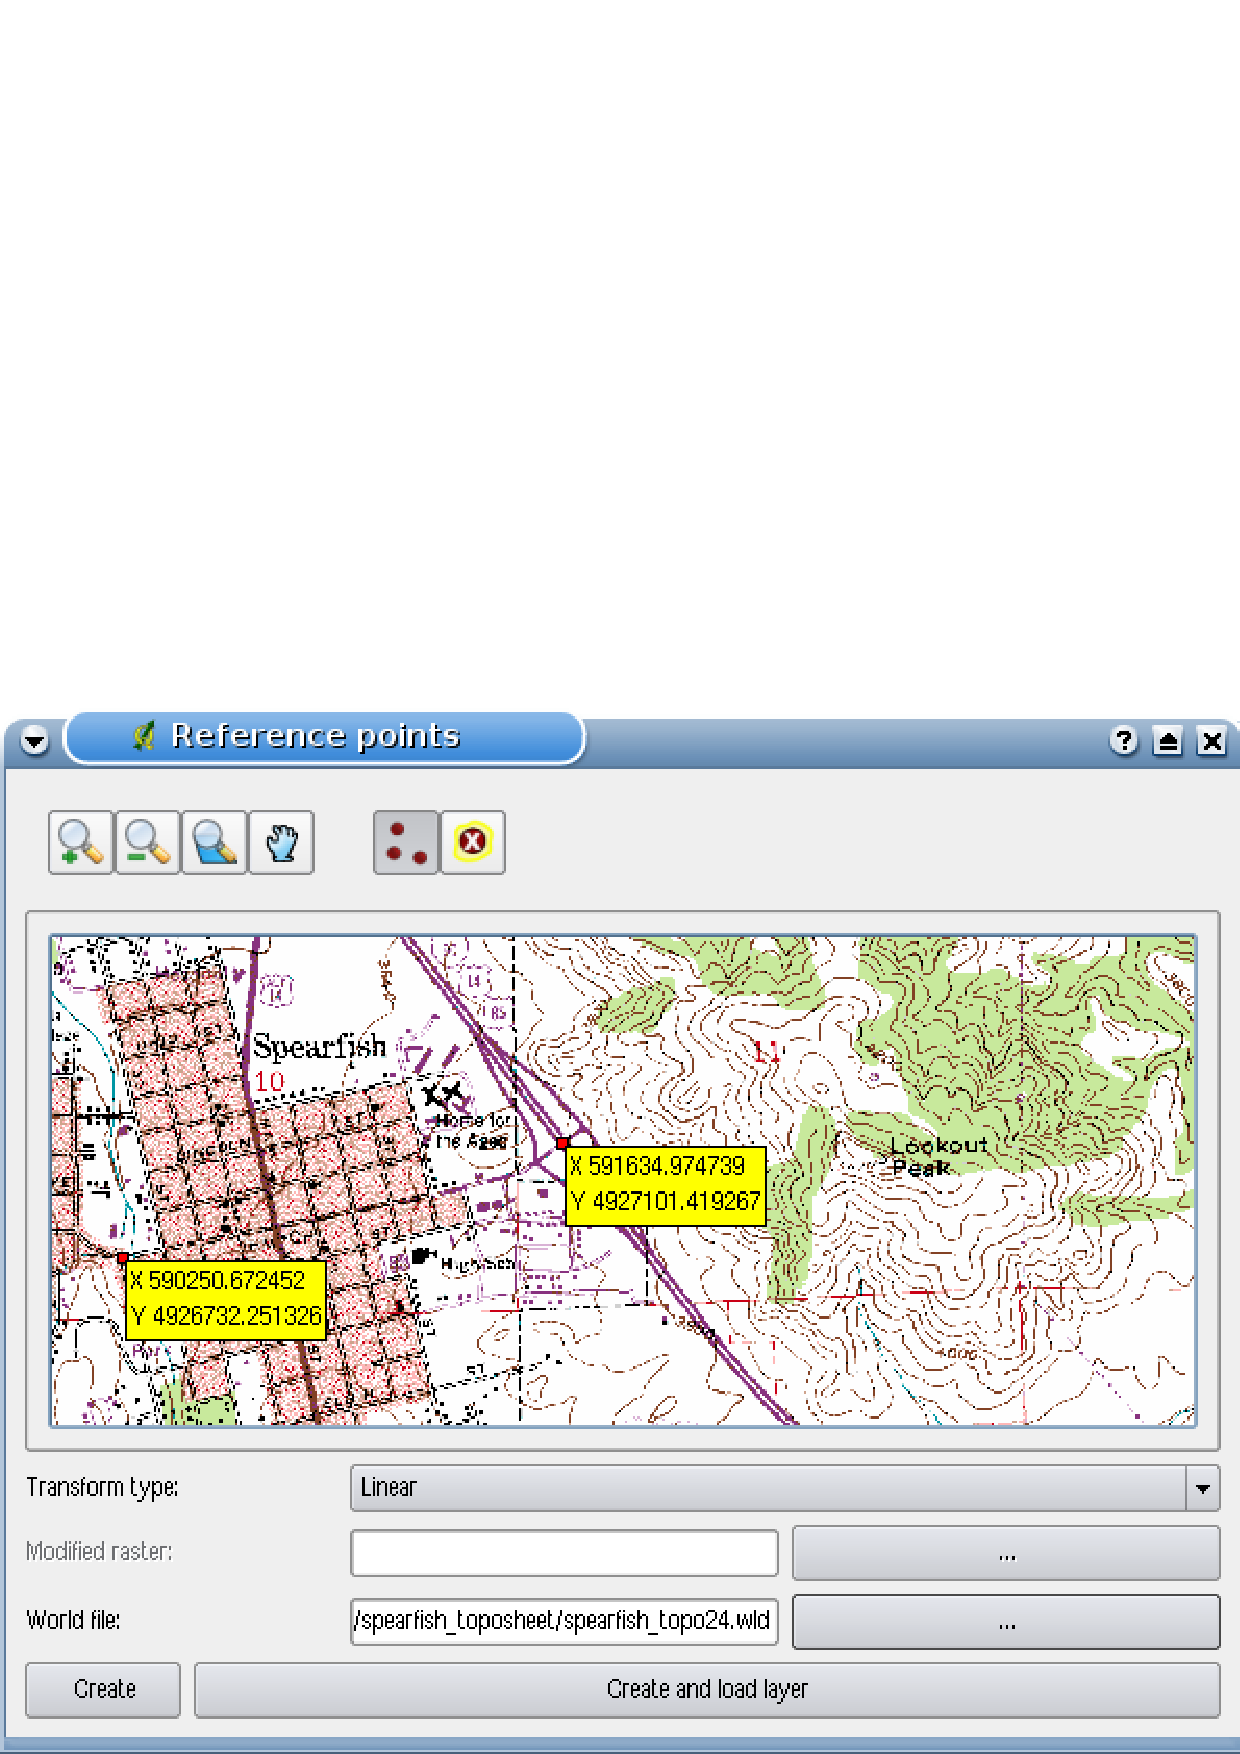
\includegraphics[clip=true,width=9cm]{choose_points}
  \caption{Добавление точек на растре \nixcaption}\label{fig:choose_points}
\end{figure}

Точки, добавленные на карту, сохраняются в отдельный текстовый файл
([имя файла].points), обычно в одном каталоге с растровым изображением.
Это дает возможность повторно загрузить модуль привязки растров позже и
добавить новые точки или удалить существующие для получения лучшего
результата. Файл с точками содержит значения формы: mapX, mapY, pixelX,
pixelY. Можно использовать кнопки

\includegraphics[width=0.7cm]{mActionFileOpen} <<Загрузить контрольные точки>> и

\includegraphics[width=0.7cm]{mActionFileSave} <<Сохранить котрольные точки>>
для изменения этих файлов.

\minisec{Определение параметров трансформации}\label{georeferencer_transformation}

После того, как контрольные точки добавлены на растровое изображение,
необходимо определить параметры преобразования для привязки.

\begin{figure}[ht]
\centering
  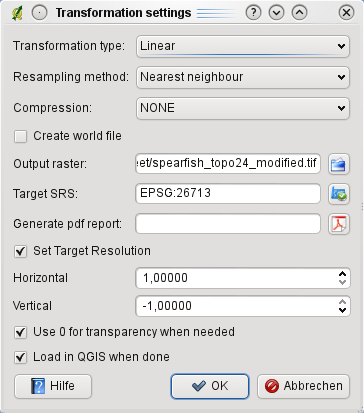
\includegraphics[clip=true,width=8cm]{transformation_settings}
  \caption{Определение параметров трансформации модуля привязки \nixcaption}\label{fig:georef_transform}
\end{figure}

\minisec{Доступные алгоритмы преобразования}

В зависимости от того, как много контрольных точек отмечено, можно
использовать различные алгоритмы преобразования. Выбор необходимого
алгоритма также зависит от типа и качества входных данных, а также
объема геометрического искажения, вносимого в конечный результирующий
файл.

На текущий момент доступны следующие алгоритмы:

\begin{itemize}[label=--]
\item \textbf{Линейный алгоритм} применяется для создания файла
привязки; его отличие от других алгоритмов заключается в том, что он
фактически не изменяет сам растр. Этот алгоритм, скорее всего, не будет
достаточным в случае, если вы работаете с отсканированным материалом.
\item \textbf{Трансформация Хельмерта} совершает простые трансформации
с изменением масштаба и вращением.
\item \textbf{Многокомпонентные алгоритмы} 1-3 порядка являются
наиболее широко используемыми алгоритмами привязки и каждый отличается
друг от друга степенью искажения, внесенного для того, чтобы
соответствовать исходнику, и целевыми контрольными точками. Самый
применяемый многокомпонентный алгоритм "--- это трансформация второго
порядка, которая допускает определенное искривление. Преобразование
первого порядка (афинное) сохраняет коллинеарность и допускает только
вращение, перевод и масштабирование.
\item \textbf{Алгоритм тонкостенного сплайна} "--- более современный
метод привязки, дающий возможность ввода в данные местных деформаций.
Данный алгоритм очень полезен, когда необходимо привязать растры с
низким качеством изображения.
\end{itemize}

\minisec{Определение метода пересчета}

Выбранный тип пересчета будет, скорее всего, зависеть от исходных данных
и конкретной цели операции. Если вы не желаете менять совокупную
информацию изображения, вам, возможно, подойдет метод <<ближайший сосед>>,
тогда как кубический пересчет приведет к более сглаженному результату.

Вот пять различных методов пересчета.

\begin{enumerate}
\item Ближайший сосед
\item Линейный
\item Кубический
\item Кубический сплайн
\item Ланцоша
\end{enumerate}

\minisec{Определение выходного растра}

Существует несколько параметров, которые необходимо определить для
привязанного растра.

\begin{itemize}[label=--]
\item Флаг \checkbox{Создать файл привязки} становится доступным, если
вы решили использовать тип линейной трансформации, потому, что это
означает, что растровое изображение фактически изменяться не будет.
В таком случае, поле <<Целевой растр>> не активируется потому, что
будет созданый новый файл привязки.
\item Для всех остальных типов трансформации нужно указать
\textbf{Целевой растр}. По умолчанию, в каталоге с исходным растровым
изображением будет создан новый файл ([имя файла]\_modified).
\item Следующим шагом будет определение \textbf{Целевая система координат}
для привязанного растра (см. раздел~\ref{label_projections}).
\item По желанию можно \textbf{Создать PDF-отчет}. Он включит
информацию об использованных параметрах трансформации, изображение
невязки и список всех контрольных точек и их среднеквадратических ошибок.
\item Кроме того, можно активировать флаг
\checkbox{Задать целевое разрешение} и определить пиксельное разрешение
для выходного растра. По умолчанию разрешение по горизонтали и вертикали
равно 1.
\item Флаг \checkbox{Использовать 0 для прозрачности при необходимости}
может активироваться, если пиксели со значение 0 должны быть показаны
прозрачными. В приведенном примере на топографической карте все белые
области будут прозрачными.
\item И наконец флаг \checkbox{Открыть результат в QGIS} загружает
выходной растр автоматическ в QGIS, когда трансформация завершена.
\end{itemize}

\minisec{Запуск преобразования}\label{georeferencer_running}

После того, как собраны все контрольные точки и заданы все параметры для
трансформации, нажмите кнопку 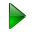
\includegraphics[width=0.7cm]{mActionStartGeoref}
<<Начать привязку>> для того, чтобы создать новый привязанный растр.
